\documentclass[a4paper]{article}
\usepackage[margin=20mm]{geometry}
\usepackage{amsmath,graphicx,booktabs}
\usepackage[hidelinks]{hyperref}

\title{Classical and Quantum-Assisted Search for QOBLIB Portfolio Optimization}
\author{Quantum Icing Team}
\date{}

\begin{document}
\maketitle

\begin{abstract}
We minimize QOBLIB's multiperiod portfolio objective over the complete benchmark: 352 configurations,
from 3 assets and 2 periods up to 400 assets and 15 periods, each checked by the official referee.
Exact methods prove 184 of them optimal: dynamic programming (DP) over all feasible period states
for every instance with at most ten assets, and an exact mixed-integer linear program (MILP) for all 44
risk-free (\(\lambda=0\)) configurations, including the 400-asset, 15-period instance.
For larger instances, a new solver combines per-period candidate pools, an exact sequence DP and
neighbor-aware re-solves. It improves the published best-known value (BKV) on all eight 50-asset instances at
\(\lambda=10^{-2}\), by up to 416\%, and on 11 further 50-asset configurations.
At 200 and 400 assets it reaches \(-842{,}939\) and \(-3{,}169{,}074\) on the two leaderboard targets.
On ten assets, three Pauli correlation encoding (PCE) search chains reach their optima using at most nine simulated qubits.
Three further quantum subroutines, tested against classical controls with the same budget, gave no improvement on the large instances. We report why.
\end{abstract}

\section{Problem formulation}

In QOBLIB's model~\cite{qoblib}, for each period \(t=0,\ldots,T-1\) and asset \(i=1,\ldots,n\), the decision consists of long and short holdings
\(L_{ti},S_{ti}\in\{0,1,2,3\}\). Set \(v_t=L_t-S_t\). The benchmark counts units of holdings, with a limit \(B\)
per period and a capital register \(C=10\). Its constraints are
\begin{equation}
\label{eq:constraints}
\sum_i(L_{ti}+S_{ti})\le B,\qquad
0\le C-\sum_i v_{ti}\le15 .
\end{equation}
The benchmark uses \(B=3,4,4,4,20,50,100\) for \(n=3,4,5,10,50,200,400\) assets.

The objective combines risk, return, cash interest, short holding fees, and transaction costs.
Let \(R_t(\lambda)\), \(r_t\), \(c_t\), and \(h_t\) be the benchmark's integer-rounded risk, return, transaction,
and short-fee coefficients. With \(C=10\), cash interest contributes \(-10(C-\sum_i v_{ti})\) per period.
Writing the objective in the benchmark's units gives
\begin{equation}
\label{eq:objective}
\begin{aligned}
F(L,S)={}&\sum_{t=0}^{T-1}
\left[v_t^\mathsf{T}R_t(\lambda)v_t+h_t^\mathsf{T}S_t
      -10\left(C-\sum_i v_{ti}\right)\right]
-\sum_{t=0}^{T-2}r_t^\mathsf{T}v_t\\
&+c_0^\mathsf{T}(L_0+S_0)+c_{T-1}^\mathsf{T}(L_{T-1}+S_{T-1})\\
&+\sum_{t=1}^{T-2}c_t^\mathsf{T}
\left(|L_t-L_{t-1}|+|S_t-S_{t-1}|\right).
\end{aligned}
\end{equation}
The separate final-period charge follows the official scorer. We minimize \(F\).
Risk coefficients are rounded after multiplication by \(\lambda\), using the benchmark's rounding convention.
Consequently, the integer coefficient tables must be rebuilt for each risk weight.
Two facts are used throughout. There is no rebalancing charge from period \(T-2\) to \(T-1\) and no return in
period \(T-1\), so an empty final period is optimal. Cash interest is linear in the net holdings, so the binary
cash register of the reference model is not needed.

\section{Exact methods}

\subsection{Dynamic programming on up to ten assets}

Holding both a long and a short position in the same asset is dominated. Replacing each pair by its net holding
preserves return, risk, and capital, decreases the number of open units, and cannot increase the holding or transaction costs.
We therefore enumerate net holdings \(v\in\{-3,\ldots,3\}^{n}\) subject to \(\sum_i|v_i|\le B\).
For \(n=10,B=4\), this gives 8,341 feasible period states. The capital constraint is automatic because
\(-4\le\sum_i v_i\le4\).

Let \(g_t(v)\) include the costs of holding \(v\) in period \(t\), including any initial or final charge.
The cost of changing holdings is kept separate. Define \(w_t=c_t\)
for \(1\le t\le T-2\) and \(w_{T-1}=0\). The recurrence is
\begin{equation}
\label{eq:dp}
D_0(v)=g_0(v),\qquad
D_t(v)=g_t(v)+\min_{u\in\mathcal V}
\left[D_{t-1}(u)+w_t^\mathsf{T}|v-u|\right].
\end{equation}
Backtracking from \(\min_v D_{T-1}(v)\) recovers the full portfolio.
The implementation sorts predecessor costs so a transition evaluation can stop once its accumulated cost
cannot improve the current minimum.

We ran \eqref{eq:dp} on all eight ten-asset instances, covering ten or fifteen periods and four market-data variants,
at each of the eight benchmark risk weights. All 64 objectives match the published reference values.
QOBLIB labels 14 of these references optimal. For the other 50, our optimality classification follows
from the exhaustive state enumeration and exact recurrence, with each recovered portfolio checked by the referee.
The same recurrence solves all 96 configurations with three to five assets (63, 313 and 671 feasible period states).
It agrees with the referee's brute force wherever that applies.

\subsection{Exact MILP for the risk-free configurations}

At \(\lambda=0\) the quadratic risk term vanishes and \eqref{eq:objective} is linear in \(L\), \(S\) and auxiliary
variables \(a_{ti}\ge|L_{ti}-L_{t-1,i}|\), \(b_{ti}\ge|S_{ti}-S_{t-1,i}|\), which enter the objective with positive costs.
With the per-period constraints \eqref{eq:constraints} this is a small MILP with \(2nT\) bounded integer variables,
for example 12,000 for 400 assets and 15 periods. HiGHS solves each of the 44 configurations to zero optimality gap in about a second.
The 400-asset, 15-period result is \(F=-4{,}194{,}965\). This is the proven optimum, below the best leaderboard
entry for that configuration (\(-4{,}194{,}749\)).

\clearpage
\section{Classical search beyond ten assets}

\subsection{Candidate pools and exact neighborhood search (earlier solver)}

As the number of assets grows, enumerating every feasible period state becomes expensive.
Our earlier solver builds a pool of candidate holdings from rounded continuous relaxations, descent over single
and paired unit moves, iterated local search, and simulated annealing. During pool construction, it explores
several approximations to entry and exit costs by charging zero, one, or two times the period's transaction
coefficient. It then uses \eqref{eq:dp} to choose a sequence from that pool with the original transaction costs.
This step optimizes the sequence over the pool, so its quality depends on the available holdings.
Large-neighborhood search (LNS) refines the result by fixing all but \(k\le4\) assets and solving
those \(k\) trajectories jointly over the full horizon by DP, with at most \(7^k\) states per day.

\subsection{Asset-trajectory DP and day-level tabu search (first campaign)}

The first campaign's solver alternates between two views of a full portfolio.
In the first, one or two assets can change across all days, and exact DP solves these subproblems over 7 or 49
states per day. In the second, every asset can change on one day while neighboring days are fixed. The tabu search
scans feasible one-unit changes to one asset or a pair. For a change \(\delta\) to the day's net holdings \(v_t\),
the risk contribution changes by
\[
\delta^\mathsf{T}(R_t+R_t^\mathsf{T})v_t+\delta^\mathsf{T}R_t\delta .
\]
Maintaining \((R_t+R_t^\mathsf{T})v_t\) makes each candidate's risk change inexpensive to evaluate.
The best admissible move can temporarily increase the objective, and reversing a recent move is blocked for several iterations.
These daily moves build hedges involving several assets that single-asset descent cannot reach.
Parallel tempering (PT) with 12 replicas and interval block moves completed the campaign.

\subsection{Day pools, exact sequence DP and neighbor-aware re-solves (new solver)}

The new solver returns to the pool-and-sequence idea of the earlier solver. It builds the pools from much stronger
day-level searches and refines the sequence with re-solves that account for neighboring days.
\begin{enumerate}
\item \textbf{Day and hold pools.} For every period \(t\) we minimize the single-period cost
\(v^\mathsf{T}R_tv+\sum_i f_{ti}(v_i)\) under \eqref{eq:constraints}, where the tables \(f_{ti}\) collect return,
fee, interest and, when neighbors are given, rebalancing costs. The search is iterated tabu search over single- and
pair-unit moves with exact integer deltas, random restarts and kicks. For more than 150 assets, pair moves are restricted to
the 40 best single moves (candidate lists). We also solve \emph{hold blocks}: one vector kept over
2--5 consecutive periods. Its risk matrix and cost tables are the sums over the block, and there is no internal rebalancing.
Elite states of every search enter the pools.
\item \textbf{Exact sequence DP.} Recurrence \eqref{eq:dp} restricted to the pools selects one state per period
with the true transaction costs. A pruned implementation keeps 150--300 states per period.
\item \textbf{Neighbor-aware re-solves.} Each period is re-solved with its neighbors fixed. Its rebalancing costs to the
neighboring periods are weighted by 1 or by \(0.5\); the latter anticipates partial holding. Random hold blocks are re-solved
in the same way. New states go into the pools and the sequence DP is rerun.
\end{enumerate}
The day searches run in parallel worker processes. Independent runs merge their incumbents through the shared
solution files, and every file is saved only if the referee confirms a strict improvement.
A final polisher alternates exact one- and two-asset trajectory DP with a full-horizon tabu search that adds
or removes one unit over a run of up to three consecutive days, alone or paired with a second asset on the same run.

\clearpage
\section{Classical results}

All 352 configurations have a referee-checked solution file. Table~\ref{tab:classical} lists the 50-asset configurations
whose objective is below the published BKV. Of the 64 fifty-asset configurations, 19 are below the BKV, 45 match it, and none is above it.
The first campaign's results (\(-50{,}971\) and \(-19{,}785\), the two largest reductions in its own table, about 61\%)
were superseded by the new solver.

\begin{table}[htbp]
\centering
\caption{Fifty-asset configurations below the published BKV (\(B=20\)). Names omit \texttt{po\_a050\_}.
Reduction is \((F_{\rm ref}-F)/|F_{\rm ref}|\). Earlier best is the first campaign's value where it beat the BKV.}
\label{tab:classical}
\begin{tabular}{@{}llrrrr@{}}
\toprule
Instance & \(\lambda\) & Published BKV & Earlier best & New solver & Reduction\\
\midrule
\texttt{t10\_s01}  & \(10^{-2}\) & \(-2{,}248\)  & ---           & \textbf{-11,605} & 416.24\%\\
\texttt{t10\_s00}  & \(10^{-2}\) & \(-12{,}340\) & \(-19{,}785\) & \textbf{-51,429} & 316.77\%\\
\texttt{t15\_orig} & \(10^{-2}\) & \(-31{,}504\) & \(-50{,}971\) & \textbf{-84,973} & 169.72\%\\
\texttt{t15\_s01}  & \(10^{-2}\) & \(-13{,}706\) & ---           & \textbf{-30,925} & 125.63\%\\
\texttt{t15\_s02}  & \(10^{-2}\) & \(-40{,}622\) & \(-41{,}517\) & \textbf{-86,212} & 112.23\%\\
\texttt{t15\_s00}  & \(10^{-2}\) & \(-43{,}792\) & ---           & \textbf{-83,001} & 89.54\%\\
\texttt{t10\_s02}  & \(10^{-2}\) & \(-43{,}565\) & \(-45{,}069\) & \textbf{-70,439} & 61.69\%\\
\texttt{t10\_orig} & \(10^{-2}\) & \(-37{,}107\) & ---           & \textbf{-53,492} & 44.16\%\\
\texttt{t15\_s01}  & \(10^{-3}\) & \(-243{,}245\) & ---          & \textbf{-243,919} & 0.277\%\\
\texttt{t10\_s00}  & \(10^{-3}\) & \(-191{,}879\) & ---          & \textbf{-192,036} & 0.082\%\\
\texttt{t15\_s02}  & \(10^{-3}\) & \(-316{,}799\) & ---          & \textbf{-316,930} & 0.041\%\\
\texttt{t10\_s01}  & \(10^{-3}\) & \(-141{,}376\) & ---          & \textbf{-141,431} & 0.039\%\\
\texttt{t15\_s00}  & \(10^{-3}\) & \(-314{,}736\) & ---          & \textbf{-314,848} & 0.036\%\\
\texttt{t15\_orig} & \(10^{-3}\) & \(-321{,}907\) & ---          & \textbf{-321,964} & 0.018\%\\
\texttt{t10\_s00}  & \(5\cdot10^{-4}\) & \(-234{,}259\) & \(-234{,}696\) & \textbf{-234,783} & 0.224\%\\
\texttt{t15\_s02}  & \(5\cdot10^{-4}\) & \(-392{,}668\) & \(-392{,}723\) & \textbf{-392,810} & 0.036\%\\
\texttt{t15\_s01}  & \(5\cdot10^{-4}\) & \(-304{,}289\) & ---          & \textbf{-304,360} & 0.023\%\\
\texttt{t15\_orig} & \(5\cdot10^{-4}\) & \(-397{,}497\) & ---          & \textbf{-397,568} & 0.018\%\\
\texttt{t10\_s01}  & \(5\cdot10^{-4}\) & \(-183{,}574\) & ---          & \textbf{-183,601} & 0.015\%\\
\bottomrule
\end{tabular}
\end{table}

\begin{figure}[htbp]
\centering
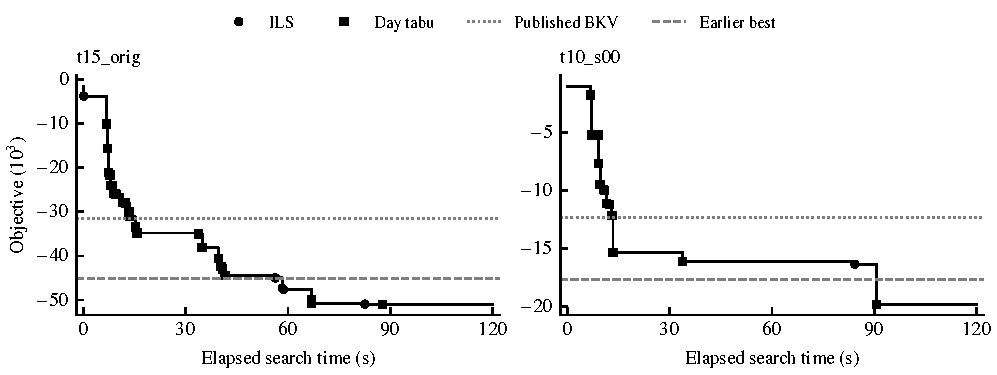
\includegraphics[width=\linewidth]{figures/portfolio-classical-progress.pdf}
\caption{First campaign: incumbent objectives for its two largest reductions, both from empty holdings at
\(\lambda=10^{-2}\). Markers identify which phase produced each improvement. Horizontal lines mark the published BKV
and the team's best before that campaign. The new solver lowers both endpoints further (Table~\ref{tab:classical}).}
\label{fig:classical}
\end{figure}

Re-solving the period problems was decisive at \(\lambda=10^{-2}\). The first campaign's portfolios left 4--7 of
the trading days empty, although a full hedged day is worth \(-5{,}000\) to \(-19{,}000\) and moving 20 units in or out costs about 2,000.
On \texttt{t15\_orig} the new solver passed the first campaign's best within 30 seconds of starting from its pools.
Several refinements found nothing when applied to the new incumbents: exact one- and two-asset trajectory DP, Gurobi
re-solves of up to 66-asset subsets of a day, and the multi-day run-move tabu. The incumbents are therefore locally optimal
for every neighborhood we implemented. On \texttt{t10\_s00} at \(\lambda=5\cdot10^{-4}\), a convex MIQP proves every
period optimal given its neighbors in under 0.4 seconds, which supports the value \(-234{,}783\) found independently by another team.

\begin{table}[htbp]
\centering
\caption{Large configurations (no published BKV). Leaderboard is the best competing entry at the time of writing.}
\label{tab:large}
\begin{tabular}{@{}lrrrl@{}}
\toprule
Instance & Earlier team best & New & Leaderboard & Method\\
\midrule
\texttt{a200\_t10\_orig}, \(\lambda=10^{-3}\) & \(-818{,}362\) & \textbf{-842,939} & \(-840{,}155\) & new solver\\
\texttt{a400\_t15\_orig}, \(\lambda=10^{-3}\) & \(-2{,}986{,}716\) & \textbf{-3,169,074} & \(-3{,}162{,}386\) & new solver + polisher\\
\texttt{a400\_t15\_s00}, \(\lambda=10^{-3}\) & \(-2{,}596{,}045\) & \(-2{,}800{,}544\) & \(-2{,}813{,}400\) & new solver (16 min)\\
\texttt{a400\_t10\_orig}, \(\lambda=10^{-3}\) & \(-1{,}896{,}257\) & \textbf{-1,994,776} & --- & new solver\\
\texttt{a400\_t15\_orig}, \(\lambda=0\) & \(-4{,}192{,}133\) & \textbf{-4,194,965} & \(-4{,}194{,}749\) & exact MILP (optimal)\\
\bottomrule
\end{tabular}
\end{table}

At 200 and 400 assets the incumbent rotates almost every unit every day. On \texttt{a200\_t10\_orig} the transaction
costs total about 78,000, so the gains come from the neighbor-aware re-solves and the half-weight variants rather than
from better isolated days. On \texttt{a400\_t15\_orig} the multi-day run moves of the polisher found the last 2,300 units
that moved the result past the leaderboard value. The full notebook QUBO for this instance would have 36,165 binary
variables. The search works with integer net holdings and uses zero qubits.

\clearpage
\section{Quantum large-neighborhood search}

\subsection{Compact portfolio QUBO}

The quantum search encodes holdings with three unary copies for each asset, direction, and period.
For example \(L_{ti}=\sum_{m=1}^{3}x^+_{tim}\), with an analogous expression for \(S_{ti}\).
A binary register \(b_t\) holds the unused budget. The objective includes the penalty
\[
W\sum_t\left[\sum_{i,m}(x^+_{tim}+x^-_{tim})
              +\sum_{j=0}^{b-1}2^j b_{tj}-B\right]^2,
\qquad b=\lceil\log_2(B+1)\rceil .
\]
For \(B=4\), the capital rule cannot bind, so cash interest is folded into the linear objective
and its four-bit slack register is removed. This gives \(6nT+bT=630\) binary variables for ten assets and ten periods,
compared with 710 in the starter encoding. Sampled assignments are decoded to net holdings and always evaluated with
the referee's count-based objective.

\subsection{Conditional windows and PCE}

At each iteration we choose a small window of asset-period cells, including the slack registers of the free periods,
and substitute the incumbent values for every variable outside the window.
If the full penalized quadratic objective is
\[
E(x)=c+\sum_i a_ix_i+\sum_{i<j}Q_{ij}x_ix_j ,
\]
then the free variable \(i\) receives linear coefficient
\(a_i+\sum_{j\notin\mathcal W}Q_{ij}\bar x_j\), interpreting \(Q\) symmetrically.
The resulting conditional QUBO is scaled by its largest absolute coefficient. The penalty weight is \(W=5000\).

Pauli correlation encoding (PCE) represents binary decisions using the signs of Pauli expectation values~\cite{pce}.
Several decisions can be extracted from one register, allowing a window with 27--42 binary variables to use 7--9 qubits.
Our implementation uses Divi 0.16.2 with polynomial encoding, a soft objective with parameter 2,
three circuit layers, and a Monte Carlo optimizer with population 40 and eight iterations.
Each circuit uses 4,000 shots on the local Maestro simulator.
We decode up to 32 returned candidates, insert each into the incumbent, repair constraint violations with the referee's
greedy repair, and accept the best candidate only if its feasible objective is lower.

\clearpage
\section{PCE experiments and comparisons}

Table~\ref{tab:pce} follows three search chains on \texttt{po\_a010\_t10\_orig}, \(B=4\).
Each chain starts from the empty portfolio, whose score is \(-1000\), and passes its best portfolio to the next run.
All three reach the independently recomputed DP optimum.

\begin{table}[htbp]
\centering
\caption{PCE continuations and their final checked objectives. Qubits gives the largest simulated register in the run.
Windows and circuits are completed totals, including iterations after the optimum was first reached.}
\label{tab:pce}
\begin{tabular}{@{}lrrrrr@{}}
\toprule
\(\lambda\) & Seed & Windows & Qubits & Circuits & Final objective\\
\midrule
\(10^{-4}\) & 3 & 300 & 8 & 96,300 & \(-69{,}397\)\\
 & 7 & 400 & 9 & 128,400 & \(-69{,}482\)\\
\(5\cdot10^{-4}\) & 5 & 400 & 8 & 128,400 & \(-26{,}882\)\\
 & 10 & 500 & 9 & 160,500 & \(-27{,}044\)\\
\(10^{-3}\) & 6 & 400 & 8 & 128,400 & \(-6{,}962\)\\
 & 8 & 500 & 9 & 160,500 & \(-7{,}759\)\\
 & 15 & 1,937 & 9 & 621,777 & \(-8{,}397\)\\
\bottomrule
\end{tabular}
\end{table}

\begin{figure}[htbp]
\centering
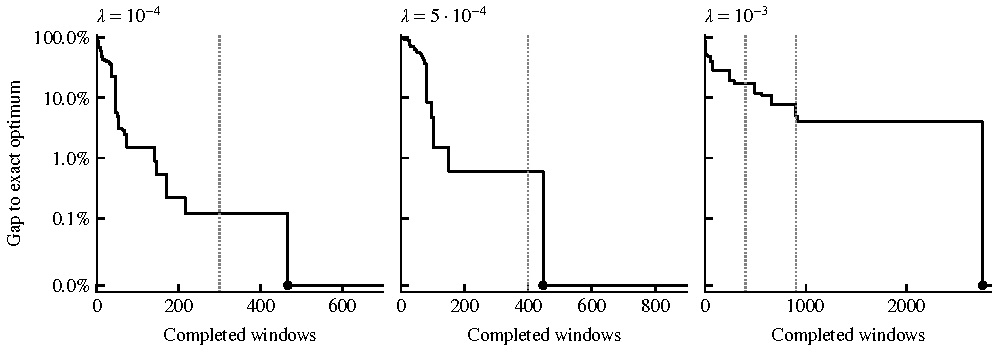
\includegraphics[width=\linewidth]{figures/portfolio-pce-progress.pdf}
\caption{Gap to the exact optimum during the three PCE chains.
Vertical dotted lines mark continuation runs, and filled dots mark the first attainment of the optimum.
The gap axis is logarithmic above 0.1\% and linear near zero.}
\label{fig:pce}
\end{figure}

The three optima first appeared after 467, 447, and 2,752 completed windows, respectively,
with 149,907, 143,487, and 883,392 circuits.
A four-layer QAOA window search, initialized with Characterization Service angles, reached \(-68{,}249\)
at \(\lambda=10^{-4}\), 1.775\% above the optimum, using up to 18 qubits and 30,200 circuits.
Partitioned QAOA followed by repair reached \(-3{,}484\), then \(-54{,}923\) after classical local search.

\subsection{Quantum subroutines inside the new classical solver}

Because the hard part of the 50-asset instances is the hedged single-period problem, we tested three quantum
subroutines there. Each was compared against classical controls with the same number of candidates or the same wall time.
\begin{itemize}
\item \textbf{PCE period solver} (100 binary variables, sign and on per asset, nine qubits with MultiBasis order-2 encoding, 37 periods
of three instances at \(\lambda=10^{-2}\)). Raw PCE states were worse than the empty portfolio in all 51 runs. After the
same 300-iteration tabu polish, PCE lost to rounded relaxations (10 wins, 23 losses), to the same loss optimized without a circuit
(13/18), and to tabu search with equal wall time (3/25). It found no period state that the controls missed. The mean-field loss
charges each undecided asset its full variance, so the relaxation collapses to the empty portfolio.
\item \textbf{PCE with a CVaR objective} on budget-safe slot and move encodings, over single periods and two-period blocks.
The sample-based loss removes the collapse, but in Divi it requires a parity encoding, whose \(2^q\) outputs (\(q\le20\)) can be
enumerated in seconds. The best output was always the starting state.
\item \textbf{Constrained QAOA windows.} A Dicke-state initial state with block-XY ring mixers keeps every sample feasible.
The cost is the exact objective change, warm-started with Characterization Service angles at its recommended six layers.
On 19--20-qubit windows, QAOA sampled the window optimum with probability \(5\cdot10^{-4}\) to \(7.4\cdot10^{-2}\),
10--400 times uniform Dicke sampling, and found it in six of six windows (uniform: one of six).
A convex MIQP, however, proves the incumbent optimal on 150 windows of 22--50 assets, mostly within 12 seconds.
A 29-qubit window takes 97 seconds to simulate at one layer.
\end{itemize}
Constrained QAOA is therefore a valid feasible-by-construction sampler with a measured advantage over random sampling.
It could not improve the new incumbents, because every window small enough to simulate is certified optimal classically faster than its circuit runs.

\clearpage
\section{Verification, interpretation, and reproduction}

The benchmark scorer recomputes each objective from the holdings in its solution file. Every one of the 352 submitted
files was rescored with the notebook's Python port of the QOBLIB referee, from exact integer coefficient tables, and is feasible.
The new solver keeps a ledger of every accepted improvement with its time, previous value and method.

The record scores above ten assets come from classical methods, and the 184 proven optima from exact DP and MILP.
The PCE chains on ten assets show that small simulated circuits can produce improving window assignments. Inside the new solver, the
quantum subroutines matched but did not beat their classical controls. The new solver, polisher and exact methods are in
\path{opus_lab/} of the team workspace. Its \path{METHODS.md} records every method with its verdict. The
quantum experiments are in \path{opus_lab/quantum/}, \path{qwin/} and \path{qpce2/}. The earlier solvers remain in
\path{portfolio_QIcing/} and \path{portfolio_search.py}.
\begin{verbatim}
cd opus_lab
python engine2.py po_a050_t15_orig 1e-2 --budget 20 --time 900 --workers 4
python milp_l0.py po_a400_t15_orig 100          # exact, lambda = 0
python exact_dp.py po_a005_t04_s01_b004_l1e-3   # exact, n <= 5
python status.py                                # referee rescoring
\end{verbatim}

\begin{thebibliography}{9}
\bibitem{qoblib}
QOBLIB.
\href{https://github.com/ZIB-AOPT/QOBLIB/tree/main/06-portfolio}{Portfolio optimization benchmark},
model, checker, and published reference objectives.

\bibitem{pce}
M. Sciorilli et al.
\href{https://doi.org/10.1038/s41467-024-55346-z}{Towards large-scale quantum optimization solvers with few qubits}.
\emph{Nature Communications}, 16, 476, 2025.
\end{thebibliography}
\end{document}
